\section{Waiting Time}
\label{sec:waitingTime}
The waiting time function is used to calculate the total time advertisers have to wait before being admitted to the topic table. 
The function directly shapes the structure of the topic table,  determines its diversity and performs flow control. 
It also protects against attacks, where a malicious actor tries to dominate the topic table and exhaust resources of the registrar. 

Each request is given a waiting time based on the IP address of the registrar, the ID of the registrar, the topic of the request and the current occupancy of the topic table. 
The waiting time function is divided into two parts: \emph{occupancy score} and  \emph{similarity score}. The final result is a product of both scores: $w =  \textit{occupancy score} \times \textit{similarity score} $. 

The \emph{occupancy score} is based uniquely on the number of the ads already in the table.
Its role is to progressively increase the waiting time as the topic table fills up and to limit the memory used by a registrar.
The \emph{occupancy score} is defined by equation~\ref{eq:occupancy}:

\begin{equation}
\label{eq:occupancy}
    \textit{occupancy score} = \frac{ba}{(1-\frac{d}{n})^{P_{occupancy}}}
\end{equation}
where $a$ is the \emph{ad lifetime} (the amount of time each ad spend in the topic table), $d$ is the number of ads in the table, $n$ is the capacity of the table. $b$ and $P_{occupacy}$ are protocol configurable parameters. 
When the number of ads in the table is low ($d \ll n$ ), the \emph{occupancy score} goes to $ba$. 
As the topic table fills up, the score will be amplified by the divisor of the equation. 
The higher values of $P_{occupancy}$, the faster the increase. 
With the current occupancy $d$ close to the capacity of the table $n$, the \emph{occupancy score} goes to infinity thus limiting the number of admitted requests. 

The role of the \emph{similarity score} is to determine how similar is the incoming request to the ads already in the topic table in terms of the IP address, the ID and the topic. 
Requests significantly different from the current content of the table receive lower similarity score resulting in lower overall waiting time. 
Such an approach promotes fairness across topics (it is easier for less popular topics to get into the table) and protects against attempts to fill the topic table by a small number of advertisers (as identified by their IP addresses and IDs). The similarity score is defined as a sum of similarity score for IP, ID and the topic of the request: $\textit{similarity score} = \textit{similarity score(IP)} + \textit{similarity score(ID)} + \textit{similarity score(topic)}$. 

The similarity score for ID and topics is the same given by the equation~\ref{eq:similarity}:
\begin{equation}
\label{eq:similarity}
    \textit{similarity score(topic)}= (\frac{d(topic)}{d})^{P_{topic}} 
\end{equation}
where $d(topic)$ is the number of ads for the specified topic already in the table, $d$ is the total number of ads in the table and $P_{topic}$ is a protocol parameter. 
The score goes to $1$ as the specified topic dominates the table $d(topic)  \approx  d$. 
Lower values of parameter $P_{topic}$ cause the similarity score to converge to $1$ faster. 

However,  for calculating the IP address diversity we use a different similarity score. 
A simple similarity score used for IDs and topics cannot be applied for IP addresses. 
An attacker may be able to generate a large number of different addresses sharing the same prefix (\eg using a single /24 IPv4 network) that, while similar, would receive low \emph{similarity scores}. 
Go Ethereum client~\footnote{https://github.com/ethereum/go-ethereum} limits the number of IP addresses coming from the same (\eg /24 IPv4 address) network. 
However,  it is impossible to reliably set those limits without knowledge about the network size or NAT configuration of honest nodes. 
Instead, we propose an approach that directly captures the similarity level across different IPs and translates it into a numerical score. 

We introduce a binary \emph{tree},  as shown on \Cref{fig:ip_tree},  that stores IP addresses used in the existing registrations in the topic table. 
Each node stores a counter,  while the edges represent consecutive $0$s or $1$s in a binary representation of IP addresses. 
For simplicity,  we present the \emph{tree} for IPv4 addresses but its adaptation for IPv6 is straightforward. 

\begin{figure}
    \includegraphics[width=0.45\textwidth]{img/ip_tree}
    \caption{Inserting an IP address into the IP \emph{tree} structure.}
    \label{fig:ip_tree}
\end{figure}

Apart from its root,  the \emph{tree} consists of 32 levels (33 levels in total) representing bits in the binary representation of IPv4 IP addresses. 
The root level is depicted as level $0$, the level of its successor as level $1$ and so on. 
The counter of every \emph{tree} node is initially set to $0$. When adding an IP to the \emph{tree},  the address is first converted to its binary representation and follows a path in the \emph{tree} corresponding to consecutive bits. 
Counters of all the visited nodes are increased by $1$. 
As a result, the root counter stores the number of all the IP addresses in the topic table, its $0$ successor stores the number of the IP addresses starting with $0$, its $1$ successor stores the number of the IP addresses starting with $1$ and so on. 
Removing an IP from the \emph{tree} follows the analogical procedure but decreases all the counters on the path. 

After each addition of an address to the \emph{tree} a score is generated.
The score is a sum of counter values of visited nodes raised to the power of the node level. 
\michal{Probably need an equation here but not sure how to write it down. Maybe @Ramin could help?} 
The counter values are taken \emph{before} the increment caused by adding the address\footnote{The first added address will thus always have a score of $0$}. 
Finally,  the similarity score for an IP is defined by:
\begin{equation}
    \textit{similarity score(IP}) = (\frac{\textit{score(IP)}}{-(\textit{rootCounter})(1 - 2^{33})})^{P_\textit{IP}}
\end{equation}
The divisor of the equation represents the maximum possible score. 
That is, a score obtained if all the IP addresses in the \emph{tree} would be the same as the one being added. 
Similarly to ID and topic score,  the IP similarity score range from $0$ to $1$ and returns values closer to 1 for different addresses sharing the same prefix (the longer the shared prefix, the higher the score).

The final formula for the waiting time function can be represented with  the following formula,  adding all \emph{similarity scores} and multiplying by the \emph{occupancy score}:

\begin{equation}
\begin{split}
    \textit{w(IP, ID, topic)} = 
    (\frac{\textit{score(IP)}}{-(\textit{rootCounter})(1 - 2^{33})})^{P_\textit{IP}} + \\
    + (\frac{d(ID)}{d})^{P_{ID}} +
    (\frac{d(topic)}{d})^{P_{topic}})
    \frac{ba}{(1-\frac{d}{n})^{P_{occupancy}}}
\end{split}
\end{equation}

The formula can be simplified like in equation~\ref{eq:simp}, where ss determines the the \emph{similarity score} and os the \emph{occupancy score}.

\begin{equation}
\label{eq:simp}
    \textit{w(IP, ID, topic)} = 
    (\textit{ss(IP)} + 
    \textit{ss(ID)} + 
    \textit{ss(topic)})
    \textit{os()}
\end{equation}

\subsection{Lower Bound}
With the waiting time formula, every change in the registrations stored in  the topic table may increase or decrease waiting times of other requests. 
Therefore,  an advertiser receiving waiting time $w(t_1)$ at time $t_1$, may get a smaller waiting time $w(t_2)$ at time $t_2$ ($t_1 < t_2$) in case the situation of the topic table is very different (\eg when an ad for the same topic expires between $t_1$ and $t_2$). 
As a result,  advertisers willing to minimize their waiting time can be incentivized to keep checking the waiting time as frequently as possible hoping for a better one.
However, this can be a problem. 
Registration ticket requests should be kept to the minimum and an incentive for constantly spamming ticket requests to get a better waiting time can overload a network and can lead to some nodes getting better performance than the rest.
Thus we designed a mechanism to avoid that any node that is already in possession of a ticket with a determined waiting time,   can get a better waiting time (including the new waiting time and the time passed between the first ticket request and the subsequent) by issuing new ticket requests.
One solution to this problem is to take into account all the expiration times when calculating the waiting time. 
However, such a solution is computationally expensive (\eg $O(n)$) and unfeasable in practice.

\begin{figure}
    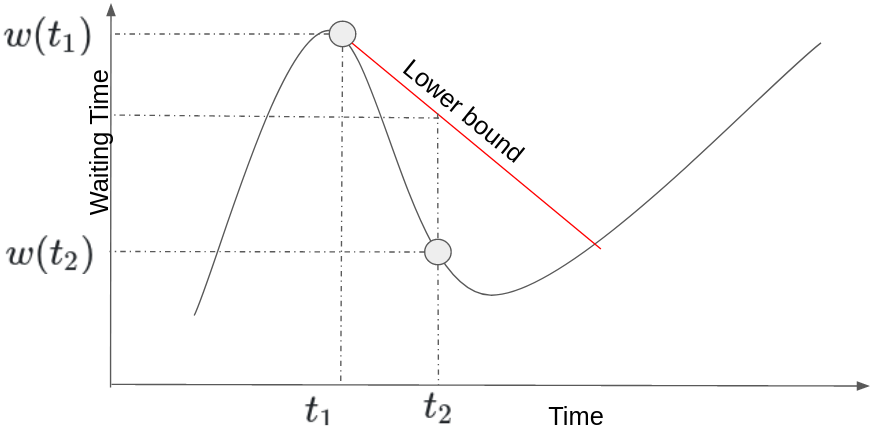
\includegraphics[width=0.45\textwidth]{img/lower_bound.png}
    \caption{Waiting time lower bound.}
    \label{fig:lower_bound}
\end{figure}

When asking for a new waiting time before the previously obtained one elapses, an advertisers loses its already accumulated waiting time . It means that asking for a new waiting at time $t_2$ can lower the overall waiting only if the new waiting time is $w(t_2)$ is smaller than $w(t_1)$ by more than $t2 - t1$: $w(t_1) - w(t_2) < t_2 - t_1$.
To make sure it is not the case,  our protocol enforces a lower bound on the waiting time. \Ie we make sure that a advertiser's waiting time received at $t_2$ is not smaller than the waiting time at $t_1$ ($t_1 < t_2$) by more than $t2 - t1$ (\Cref{fig:lower_bound}). 
However, holding such a bound for every request (\ie every combination of IP/ID/topic) would cause significant memory overhead ($O(|IPs|\times|IDs|\times|topics|)  \gg O(d)$) and would present an easy way for an attacker to create state at the registrar. 

To store the lower bound in a more efficient way, we rewrite the waiting formula as a sum of topic/IP/ID distinctive parts:

\begin{equation}
    \textit{w(IP, ID, topic)} = 
    \textit{ss(IP)}\textit{os()} + 
    \textit{ss(ID)}\textit{os()} + 
    \textit{ss(topic)}\textit{os()}
\end{equation}
Ensuring that the lower bound is enforced for each of the three components makes sure that the total waiting will respect the lower bound as well. At the same time, it only requires storing lower bound for every IP/ID/topic and not all their combinations. This approach reduces the memory overhead to $O(|IPs|+|IDs|+|topics|) = O(d)$.

For each of the components above IP, ID and topic present in the table, we keep a bound. When a specific IP enters the table for the first time, the bound(IP) is set to 0 and a timestamp timestamp(IP) is set to the current time. When a ticket request arrives from the same IP, we calculate the IP waiting time $w_{IP}$ and return the higher value among $w_{IP} = max(w_{IP}, bound(IP) - timestamp(IP))$. It makes sure that advertisers never receive a better time by frequently coming requesting new tickets. The bound and the bound are updated when a new ticket is issued and $w_{IP} > (bound(IP) - timestamp(IP))$. The same holds for IDs and topics.


